\section{\textbf{Testes do \textit{software}}}
\label{testes_do_software}
O \textit{software} criado no decorrer deste projeto é uma simples ideia de como usar técnicas de visão computacional aplicadas no reconhecimento de um jogador de futebol americano. Para exemplificar a usabilidade e os pontos fortes das técnicas utilizadas durante o desenvolvimento do mesmo, foram criadas várias situações para testar o desemprenho do algoritmo. Sendo assim, as figuras a seguir representam os testes feitos com o sistema desenvolvido.

\begin{figure}[ht]
	\caption{\label{fig_rec_numero}A imagem (A) representa os pontos de interesse encontrados nos números das camisas dos jogadores. A imagem (B) a sua identificaç ão.}
	\begin{center}
		\resizebox{1.0\linewidth}{!}{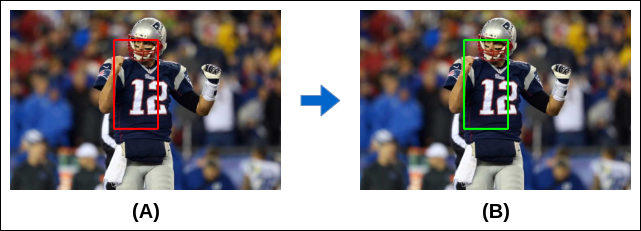
\includegraphics{6-Desenvolvimento-Projeto/imagens-desenvolvimento/representacao_numero.png}}
	\end{center}
	\centering \legend{Fonte: Elaborada pelos autores.}
\end{figure}

\begin{figure}[ht]
	\caption{\label{fig_rep_jogador_em_campo}Identificação de um jogador em uma partida de futebol americano.}
	\begin{center}
		\resizebox{.9\linewidth}{!}{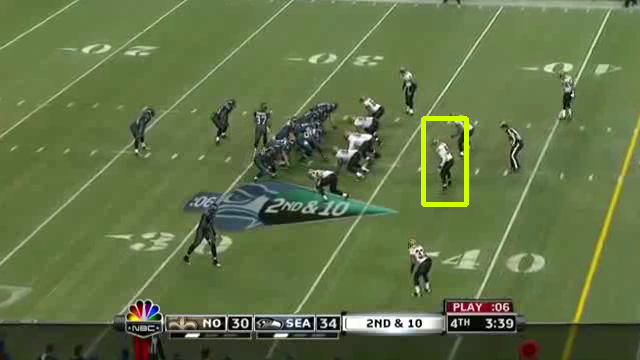
\includegraphics{6-Desenvolvimento-Projeto/imagens_teste/identificacao_jogador_em_campo_2.png}}
	\end{center}
	\centering \legend{Fonte: Elaborada pelos autores.}
\end{figure}

\begin{figure}[ht]
	\caption{\label{fig_rep_jogador_mais_evidente}Identificação do jogador mais evidente.}
	\begin{center}
		\resizebox{.9\linewidth}{!}{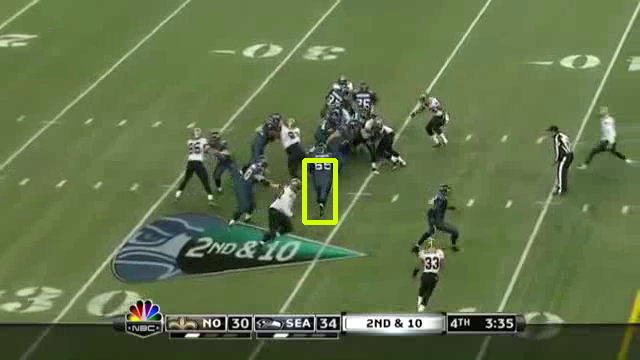
\includegraphics{6-Desenvolvimento-Projeto/imagens_teste/jogador_mais_evidente.png}}
	\end{center}
	\centering \legend{Fonte: Elaborada pelos autores.}
\end{figure}

\begin{figure}[ht]
	\caption{\label{fig_rep_jogador_em_movimento}Identificação de um jogador em movimento dentro de campo.}
	\begin{center}
		\resizebox{.9\linewidth}{!}{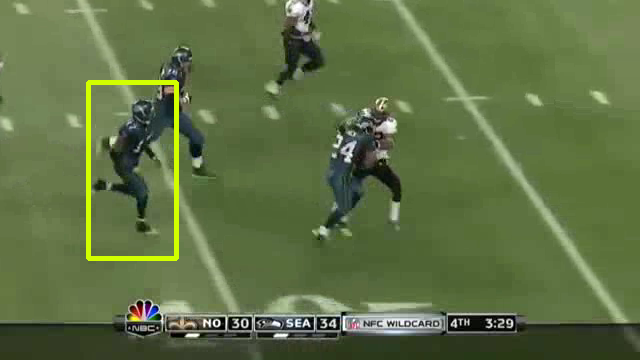
\includegraphics{6-Desenvolvimento-Projeto/imagens_teste/jogador_em_movimento.png}}
	\end{center}
	\centering \legend{Fonte: Elaborada pelos autores.}
\end{figure}

\begin{figure}[ht]
	\caption{\label{fig_rep_jogador_em_jogada}Identificação de um jogador em movimento para disputar uma jogada.}
	\begin{center}
		\resizebox{.9\linewidth}{!}{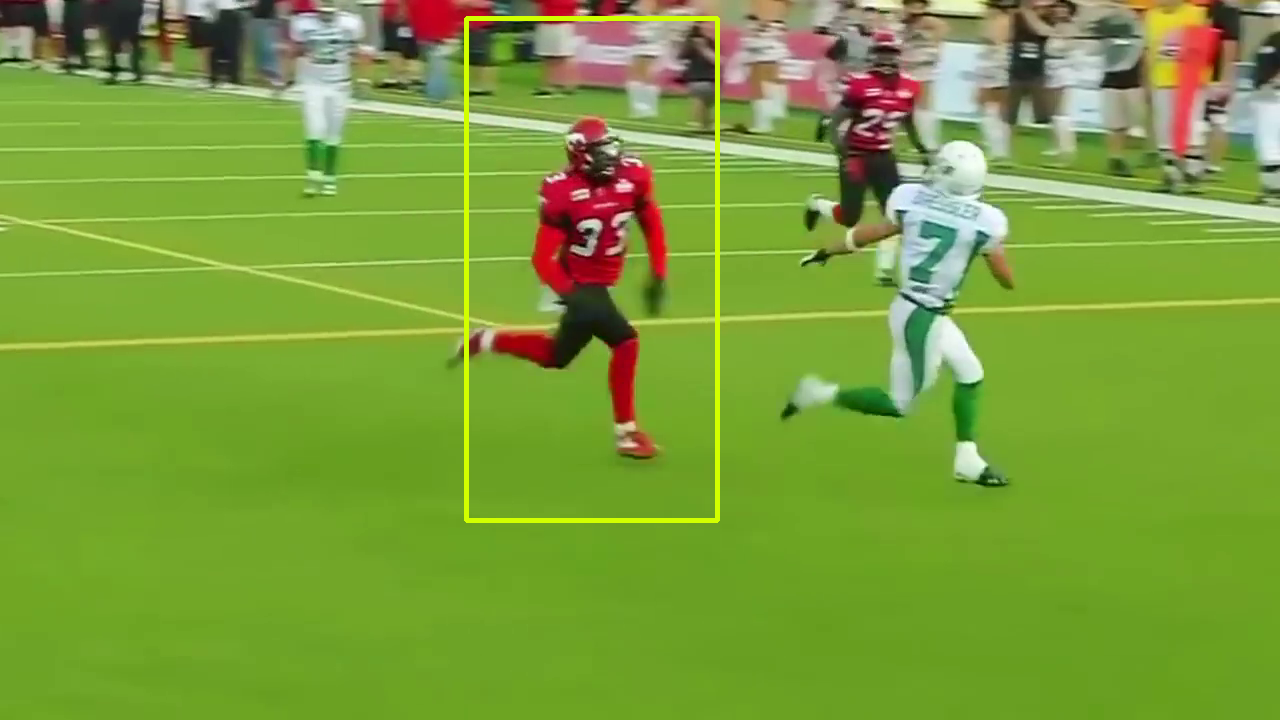
\includegraphics{6-Desenvolvimento-Projeto/imagens_teste/identificacao_jogadores_fa3.png}}
	\end{center}
	\centering \legend{Fonte: Elaborada pelos autores.}
\end{figure}

\begin{figure}[ht]
	\caption{\label{fig_rep_acessorios}Identificação dos acessórios de um jogador de futebol americano.}
	\begin{center}
		\resizebox{.9\linewidth}{!}{\includegraphics{6-Desenvolvimento-Projeto/imagens_teste/identificacao_jogadores_fa5.png}}
	\end{center}
	\centering \legend{Fonte: Elaborada pelos autores.}
\end{figure}

\begin{figure}[ht]
	\caption{\label{fig_rep_arbitro}Reconhecimento do árbitro dentro de campo.}
	\begin{center}
		\resizebox{.9\linewidth}{!}{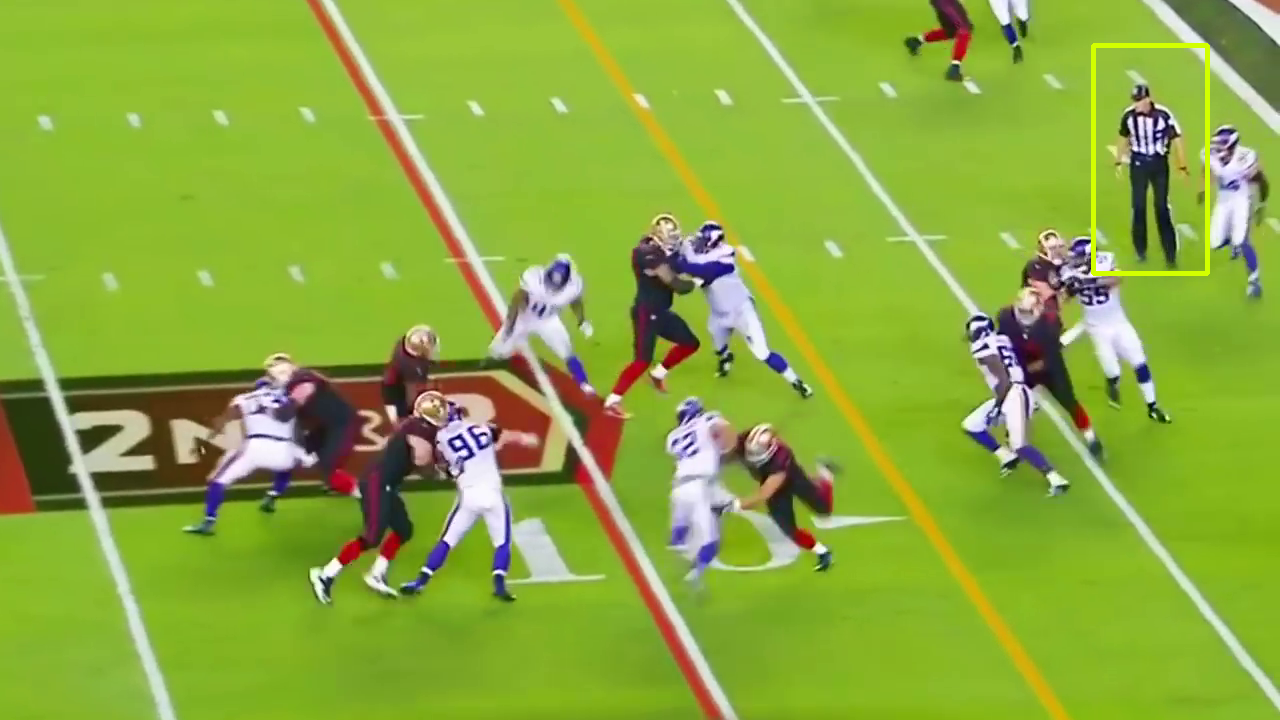
\includegraphics{6-Desenvolvimento-Projeto/imagens_teste/identificacao_arbitro.png}}
	\end{center}
	\centering \legend{Fonte: Elaborada pelos autores.}
\end{figure}

\begin{figure}[ht]
	\caption{\label{fig_processamento_maquina}Representação do processamento da máquina.}
	\begin{center}
		\resizebox{.9\linewidth}{!}{\includegraphics{6-Desenvolvimento-Projeto/imagens_teste/processamento_maquina.png}}
	\end{center}
	\centering \legend{Fonte: Elaborada pelos autores.}
\end{figure}

\clearpage